\clearpage % Start a new page
\chapter{Pruebas experimentales y análisis de resultados computacionales}
\label{sec:Pruebas experimentales y análisis de resultados computacionales}
\lhead{\emph{Pruebas experimentales y análisis de resultados computacionales}}

Este capítulo presenta el análisis de los resultados obtenidos a partir de una serie de experimentos diseñados para evaluar y mejorar progresivamente un modelo de predicción a corto plazo del nivel del río Paraguay. La estrategia parte de una configuración base basada en redes neuronales tipo GRU, cuyo potencial ya ha sido validado en estudios anteriores frente a modelos clásicos como ARIMA. A partir de esta base, se incorporan mejoras sucesivas que incluyen reentrenamiento periódico, variables hidrometeorológicas exógenas, ingeniería de características y optimización de hiperparámetros, con el objetivo de construir una arquitectura predictiva robusta y operativamente útil.

El objetivo de esta sección es comparar cuantitativa y cualitativamente cada enfoque, destacando sus fortalezas y limitaciones en función de métricas hidrológicas estándar (NSE, RMSE, MAE, MAPE). La evaluación se realiza sobre un conjunto de prueba correspondiente al periodo 2013–2022, que incluye condiciones hidrológicas variadas y años extremos como 2020 y 2021, afectados por eventos prolongados de La Niña.

El análisis se organiza en tres bloques: en primer lugar, se presenta una comparación general del desempeño en el horizonte de predicción de 28 días, considerado prioritario por su utilidad operativa. En segundo lugar, se desarrolla un estudio por configuración experimental, abarcando múltiples horizontes (7, 14, 21 y 28 días). Finalmente, se incluye un análisis detallado del comportamiento del modelo propuesto mediante visualizaciones específicas que permiten evaluar su estabilidad, sensibilidad temporal y capacidad de adaptación frente a eventos hidrológicos extremos.



\section{Desempeño en el Conjunto de Prueba}
\label{sec:desempeno_prueba}

La Tabla~\ref{tab:metricas_globales_h28} presenta las métricas globales de desempeño para cada una de las configuraciones evaluadas (Mejora 1 a 4), las cuales fueron diseñadas de forma incremental: cada nuevo experimento incorpora mejoras adicionales sobre el anterior, permitiendo analizar el impacto individual y acumulativo de cada estrategia, considerando un horizonte de predicción de 28 días y un periodo de evaluación comprendido entre enero de 2013 y diciembre de 2022. Este conjunto abarca una década completa de condiciones hidrológicas diversas, incluyendo eventos extremos como las bajantes de 2020 a 2022, asociadas al fenómeno de La Niña.

\begin{table}[H]
\centering
\caption{Métricas globales de predicción (2013–2022) para horizonte de 28 días}
\label{tab:metricas_globales_h28}
\begin{tabular}{p{4.8cm}cccc}
\toprule
\textbf{Experimento} & \textbf{NSE} & \textbf{RMSE (m)} & \textbf{MAE (m)} & \textbf{MAPE (\%)} \\
\midrule
Exp. 0 – Modelo base & 0.9177 & 0.6088 & 0.4011 & 61.71 \\
Exp. 1 – + Reentrenamiento & 0.9322 & 0.5669 & 0.3685 & 53.79 \\
Exp. 2 – + Covariables & 0.9397 & 0.5346 & 0.3538 & 41.10 \\
Exp. 3 – + Ing. de características & 0.9415 & 0.5266 & 0.3435 & 44.53 \\
Exp. 4 – + Opt. de hiperparámetros & \textbf{0.9455} & \textbf{0.5084} & \textbf{0.3126} & \textbf{30.85} \\
\bottomrule
\end{tabular}
\end{table}

A medida que se introducen mejoras en la configuración del modelo, se observa una reducción progresiva en todas las métricas de error. En particular, el error porcentual absoluto medio (MAPE) disminuye de 61.71\,\% en el modelo base a 30.85\,\% en el modelo propuesto, lo que representa una mejora relativa cercana al 50\,\%. Esta reducción es especialmente relevante para contextos donde la interpretación porcentual del error facilita la toma de decisiones prácticas y operativas.

Respecto a los errores absolutos, el RMSE se reduce de 0.6088\,m en el modelo base a 0.5084\,m en el modelo propuesto, mientras que el MAE baja de 0.4011\,m a 0.3126\,m. Estas mejoras son significativas en términos hidrológicos, ya que diferencias de medio metro pueden condicionar la navegación fluvial, el uso de puertos y el funcionamiento de obras de infraestructura ribereña.

El coeficiente de eficiencia de Nash–Sutcliffe (NSE), que mide la concordancia entre los valores observados y predichos, también mejora de forma sostenida. Partiendo de un valor inicial de 0.9177 —ya considerado adecuado para fines operativos—, se alcanza un valor final de 0.9455, lo que refleja una mayor capacidad explicativa del modelo incluso en presencia de alta variabilidad estacional.

El modelo propuesto (Experimento 4), que incorpora tanto covariables hidrometeorológicas como acumulados de precipitación seleccionados y una optimización bayesiana de hiperparámetros, consolida una arquitectura robusta para predicciones a 28 días. Su capacidad para reducir el error de forma estable a lo largo del periodo de prueba y mejorar el seguimiento de eventos extremos lo posiciona como una alternativa confiable para apoyar la toma de decisiones en gestión hídrica anticipada.



\section{Comparativa de Estrategias Experimentales}
\label{sec:comparativa_experimentos}

\subsection{Mejora 1: Reentrenamiento periódico para adaptación temporal}
\label{ssec:exp1}

Este experimento introduce un mecanismo de reentrenamiento periódico, aplicado anualmente, que permite al modelo actualizarse con los datos más recientes. A diferencia del modelo base, que se entrena una única vez sobre el conjunto histórico, esta estrategia busca mejorar la capacidad del modelo para adaptarse a cambios graduales en las condiciones hidrológicas a lo largo del tiempo.

La Tabla~\ref{tab:exp1_metricas_horizontes} presenta las métricas obtenidas para diferentes horizontes de predicción. El principal foco de análisis se centra en el horizonte de 28 días, ya que es el más relevante desde el punto de vista operativo y permite una comparación directa con el modelo base.

\begin{table}[H]
\centering
\caption{Métricas por horizonte — Experimento 1}
\label{tab:exp1_metricas_horizontes}
\begin{tabular}{lcccc}
\toprule
\textbf{Horizonte} & \textbf{NSE} & \textbf{RMSE (m)} & \textbf{MAE (m)} & \textbf{MAPE (\%)} \\
\midrule
7 días  & 0.9934 & 0.1682 & 0.1034 & 12.98 \\
14 días & 0.9791 & 0.3045 & 0.1879 & 24.04 \\
21 días & 0.9575 & 0.4421 & 0.2791 & 32.58 \\
28 días & 0.9322 & 0.5669 & 0.3685 & 53.79 \\
\bottomrule
\end{tabular}
\end{table}


En el horizonte de 28 días, el reentrenamiento periódico permite mejorar el desempeño del modelo en todos los indicadores respecto al modelo base. El NSE se incrementa de 0.9177 a 0.9322, lo que indica una mayor capacidad para explicar la variabilidad de los datos observados. Asimismo, el RMSE se reduce de 0.6088 a 0.5669 metros y el MAE baja de 0.4011 a 0.3685 metros. La mejora más significativa se observa en el MAPE, que se reduce de 61.71\% a 53.79\%, lo cual implica una menor desviación relativa promedio entre predicción y observación.

Estas mejoras reflejan el beneficio de permitir que el modelo se ajuste anualmente a nuevas condiciones del sistema, corrigiendo desviaciones acumuladas y manteniendo la precisión a lo largo de varios años de prueba.


\subsection{Mejora 2: Adición de covariables hidrometeorológicas (caudal y precipitación)}
\label{ssec:exp2}

En esta configuración experimental se incorporan variables hidrometeorológicas adicionales al modelo: caudales y precipitaciones registradas en estaciones relevantes. La motivación detrás de esta mejora es capturar dinámicas aguas arriba y fenómenos meteorológicos que afectan indirectamente el nivel del río en la estación objetivo.

La Tabla~\ref{tab:exp2_metricas_horizontes} muestra las métricas obtenidas para cada uno de los horizontes evaluados.

\begin{table}[H]
\centering
\caption{Métricas por horizonte — Experimento 2}
\label{tab:exp2_metricas_horizontes}
\begin{tabular}{lcccc}
\toprule
\textbf{Horizonte} & \textbf{NSE} & \textbf{RMSE (m)} & \textbf{MAE (m)} & \textbf{MAPE (\%)} \\
\midrule
7 días  & 0.9937 & 0.1640 & 0.1083 & 10.80 \\
14 días & 0.9811 & 0.2896 & 0.1881 & 22.60 \\
21 días & 0.9620 & 0.4179 & 0.2691 & 35.00 \\
28 días & 0.9397 & 0.5346 & 0.3538 & 41.10 \\
\bottomrule
\end{tabular}
\end{table}

Para el horizonte de 28 días, que representa el foco principal de este análisis, se evidencian mejoras sustanciales respecto al modelo base. El NSE aumenta de 0.9177 a 0.9397, indicando una mayor capacidad del modelo para reproducir la variabilidad de la serie observada. Además, el RMSE se reduce de 0.6088m a 0.5346m y el MAE baja de 0.4011m a 0.3538m.

La mejora más marcada se da en el MAPE, que pasa de 61.71\% en el modelo base a 41.10\% en este experimento, representando una reducción relativa del error porcentual superior al 33\%. Esto refleja que la inclusión de variables hidrometeorológicas aporta información relevante que permite ajustar mejor la magnitud de las predicciones, particularmente en periodos de alta variabilidad climática.

Estos resultados destacan el valor de incorporar fuentes de información exógena para capturar fenómenos que no pueden ser explicados únicamente por la evolución histórica del nivel del río.


\subsection{Mejora 3: Ingeniería de características basada en acumulados de precipitación}
\label{ssec:exp3}

En este experimento se explora el impacto de incorporar acumulados móviles de precipitación como nuevas variables explicativas. Para ello, se generaron características derivadas a partir de precipitaciones acumuladas en ventanas temporales específicas, seleccionadas mediante análisis de correlación cruzada. Esta ingeniería de características busca capturar efectos retardados de eventos lluviosos sobre el nivel del río en la estación objetivo.

La Tabla~\ref{tab:exp3_metricas_horizontes} presenta las métricas obtenidas para cada uno de los horizontes evaluados.

\begin{table}[H]
\centering
\caption{Métricas por horizonte — Experimento 3}
\label{tab:exp3_metricas_horizontes}
\begin{tabular}{lcccc}
\toprule
\textbf{Horizonte} & \textbf{NSE} & \textbf{RMSE (m)} & \textbf{MAE (m)} & \textbf{MAPE (\%)} \\
\midrule
7 días  & 0.9935 & 0.1666 & 0.1118 & 11.11 \\
14 días & 0.9796 & 0.3013 & 0.2026 & 23.22 \\
21 días & 0.9621 & 0.4171 & 0.2701 & 32.46 \\
28 días & 0.9415 & 0.5266 & 0.3435 & 44.53 \\
\bottomrule
\end{tabular}
\end{table}

En comparación con la configuración anterior (Experimento 2), se observa una mejora consistente en el horizonte de 28 días, con una reducción adicional del RMSE (de 0.5346m a 0.5266m) y del MAE (de 0.3538m a 0.3435m). Aunque el MAPE se incrementa levemente respecto al experimento anterior, el valor del NSE sigue aumentando, alcanzando 0.9415, el más alto hasta el momento en este horizonte.

Estos resultados indican que la incorporación de acumulados de precipitación, seleccionados según ventanas temporales optimizadas, permite capturar mejor la influencia gradual de las lluvias sobre el comportamiento del río. Esto se traduce en una mayor precisión del modelo a largo plazo, fortaleciendo su capacidad para representar relaciones no lineales y efectos diferidos entre variables.

La mejora, aunque sutil, es especialmente valiosa en el horizonte de 28 días, donde cada reducción marginal en el error absoluto puede marcar una diferencia significativa en contextos operativos.


\subsection{Mejora 4: Optimización bayesiana de hiperparámetros}
\label{ssec:exp4}

En este experimento final se aplica una optimización sistemática de hiperparámetros sobre el modelo, incluyendo aspectos como el tamaño de la ventana de entrada, número de unidades en la capa GRU, tasa de aprendizaje, tasa de abandono (dropout) y configuración de reentrenamiento. El proceso se llevó a cabo mediante búsqueda bayesiana, utilizando múltiples métricas como criterios de selección.

La Tabla~\ref{tab:exp4_metricas_horizontes} resume los resultados obtenidos para cada horizonte.

\begin{table}[H]
\centering
\caption{Métricas por horizonte — Experimento 4 (modelo propuesto)}
\label{tab:exp4_metricas_horizontes}
\begin{tabular}{lcccc}
\toprule
\textbf{Horizonte} & \textbf{NSE} & \textbf{RMSE (m)} & \textbf{MAE (m)} & \textbf{MAPE (\%)} \\
\midrule
7 días  & 0.9946 & 0.1512 & 0.0954 & 10.88 \\
14 días & 0.9834 & 0.2716 & 0.1636 & 17.69 \\
21 días & 0.9643 & 0.4051 & 0.2443 & 24.08 \\
28 días & 0.9455 & 0.5084 & 0.3126 & 30.85 \\
\bottomrule
\end{tabular}
\end{table}

El modelo propuesto alcanza el mejor desempeño en todos los horizontes, consolidando la mejora progresiva observada en los experimentos anteriores. En el horizonte de 28 días, que representa el foco principal del estudio, el NSE asciende a 0.9455 y el RMSE se reduce a 0.5084m, marcando una mejora significativa respecto al modelo base (0.9177 y 0.6088m, respectivamente).

Además, el MAPE cae por debajo del 31\%, una mejora de más de 30 puntos porcentuales frente al modelo base, lo cual representa un avance notable en términos de precisión relativa. También se observa una reducción constante del MAE hasta alcanzar 0.3126m, el valor más bajo entre todas las configuraciones.

Estas mejoras son el resultado combinado de las estrategias anteriores —reentrenamiento periódico e incorporación de covariables relevantes— junto con la sintonización cuidadosa de los parámetros del modelo. La versión optimizada no solo ofrece predicciones más precisas, sino que también demuestra mayor estabilidad entre horizontes, lo que la convierte en una alternativa robusta para aplicaciones operativas en escenarios reales.

\vspace{1em}
\noindent
\textbf{Resumen comparativo:} A lo largo de los cuatro experimentos realizados, se observa una mejora progresiva y sostenida en todas las métricas evaluadas para el horizonte de 28 días. El modelo base, si bien adecuado en términos generales, presenta errores porcentuales elevados y menor estabilidad temporal. La inclusión de reentrenamiento periódico permite al modelo adaptarse a condiciones cambiantes, mientras que las covariables hidrometeorológicas y la ingeniería de características mejoran su capacidad para captar relaciones físicas no lineales. Finalmente, la optimización de hiperparámetros permite consolidar estas mejoras en una arquitectura más precisa y estable. El modelo propuesto demuestra así no solo mayor precisión, sino también una degradación controlada y una capacidad de adaptación superior frente a eventos hidrológicos extremos.



\section{Análisis Detallado de Resultados}
\label{sec:analisis_resultados}

En esta sección se presentan visualizaciones específicas que permiten interpretar en mayor profundidad el desempeño del modelo propuesto, particularmente en el horizonte de predicción de 28 días. Se incluyen comparaciones visuales entre modelos, evolución del error a lo largo del tiempo, análisis por día predicho y un estudio puntual de un periodo representativo.

\subsection{Comparación Visual de Predicciones (H28)}
\label{ssec:comparacion_visual_pelos}

La Figura~\ref{fig:pelos_h28} presenta una comparación visual entre el modelo base y el modelo propuesto para el horizonte de 28 días. La línea azul continua representa los valores reales del nivel del río en la estación 86218, mientras que los puntos superpuestos muestran las predicciones generadas por ambos modelos en ventanas móviles. Los puntos rojos corresponden al modelo base, y los negros al modelo propuesto.

\begin{figure}[H]
\centering
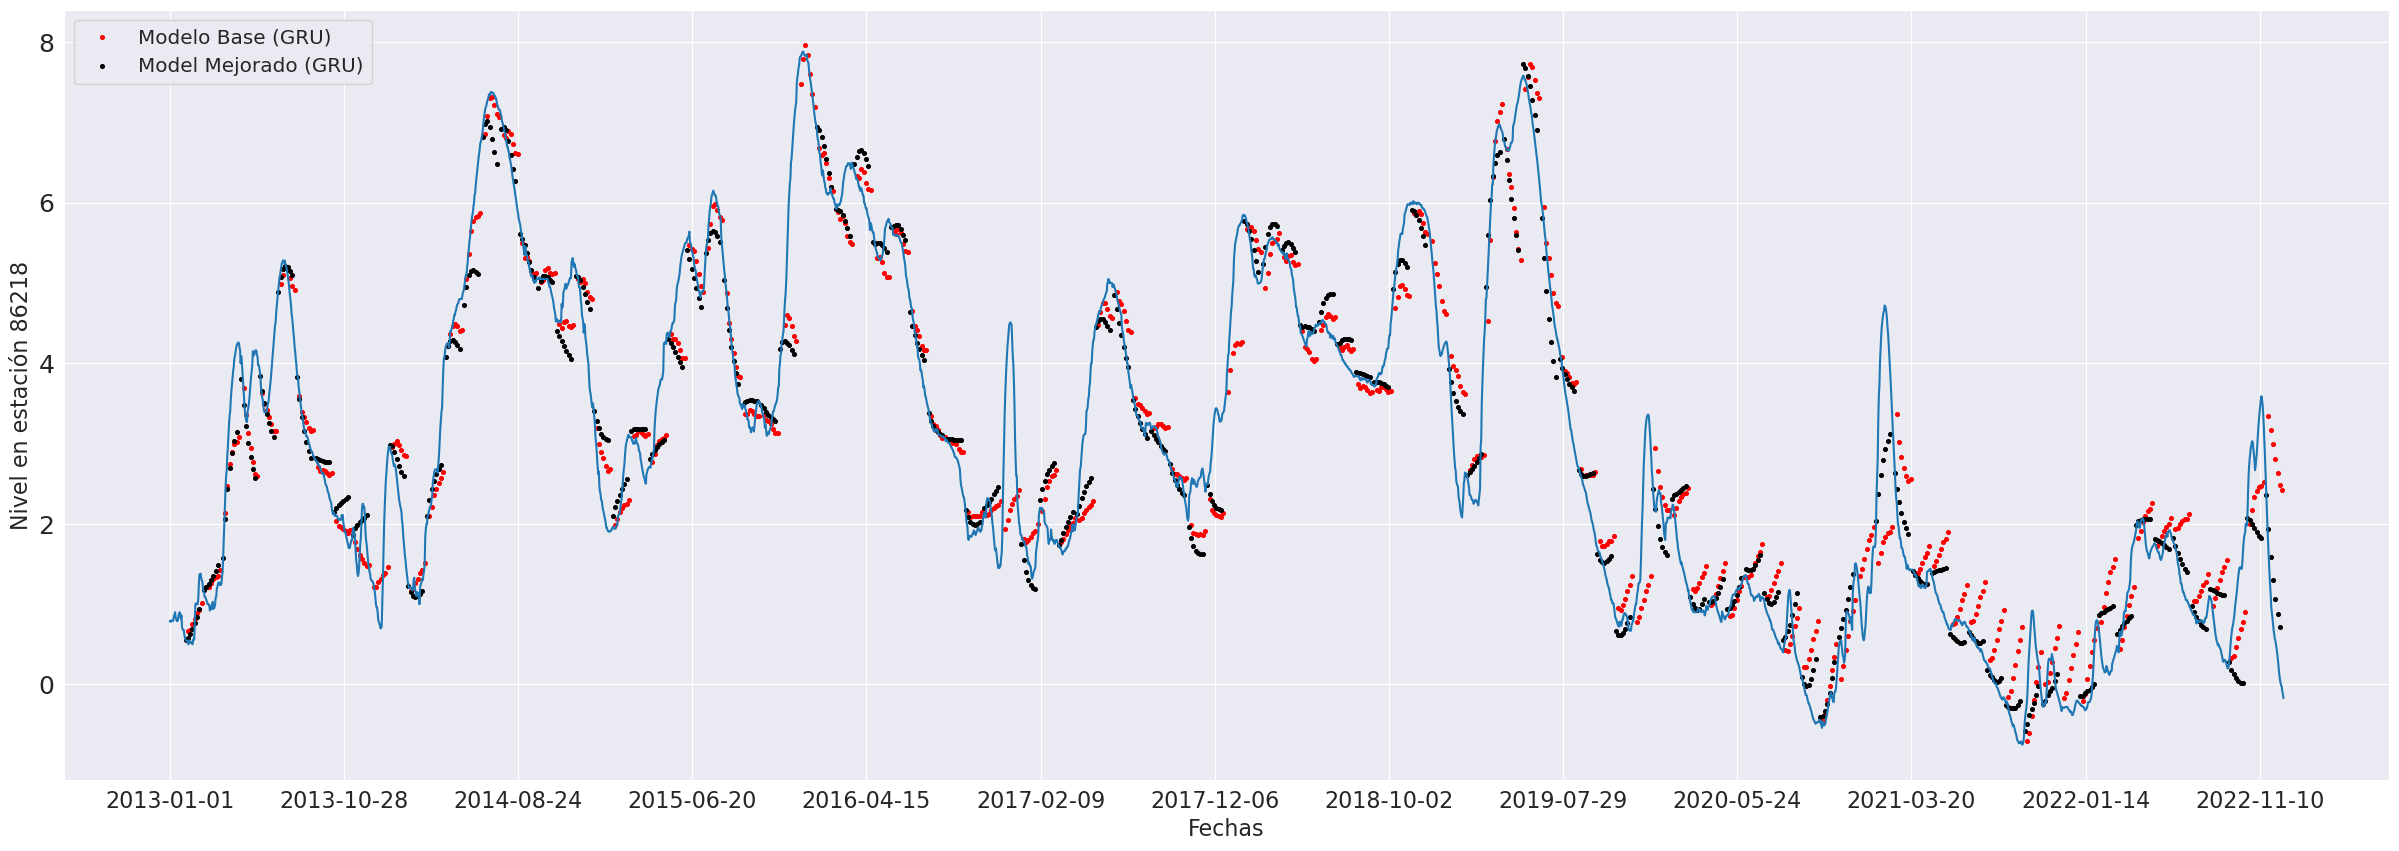
\includegraphics[width=0.95\textwidth]{Figuras/FIGURA_PARA_PEGAR.png}
\caption{Predicciones a 28 días con ventanas móviles: comparación entre el modelo base (rojo) y el modelo propuesto (negro) sobre los valores reales (línea azul).}
\label{fig:pelos_h28}
\end{figure}

La figura permite visualizar claramente cómo se comportan ambos modelos a lo largo del periodo de prueba (2013–2022). En general, el modelo mejorado (negro) presenta una mayor adherencia a la curva real, con menor dispersión y una mayor capacidad para seguir la dirección de las variaciones, especialmente durante los picos y valles.

Entre los años 2019 y 2021, por ejemplo, se observa una marcada diferencia: el modelo base tiende a dispersarse con mayor amplitud en los extremos, mientras que el modelo propuesto se ajusta con mayor precisión, capturando mejor tanto los máximos como los descensos pronunciados. Este patrón también se repite en otros tramos con alta dinámica hidrológica, como los eventos de crecida de 2014 o 2016.

La visualización \ref{fig:pelos_h28} permite evaluar no solo la precisión punto a punto, sino también la estabilidad y coherencia del modelo ante diferentes condiciones hidrológicas. El modelo propuesto muestra una distribución de predicciones más concentrada en torno a la serie real, lo cual refuerza su utilidad práctica para el monitoreo y planificación en horizontes extendidos.


\subsection{Análisis por Año: Evolución del Error (H28)}
\label{ssec:errores_por_anho}

La Figura~\ref{fig:errores_anuales} presenta la evolución interanual de las métricas NSE, RMSE, MAE y MAPE para el horizonte de 28 días, comparando el modelo anterior (base) y el modelo propuesto (final). Este análisis permite observar el comportamiento de cada modelo frente a condiciones hidrológicas cambiantes a lo largo del periodo 2013–2022.

\begin{figure}[H]
\centering
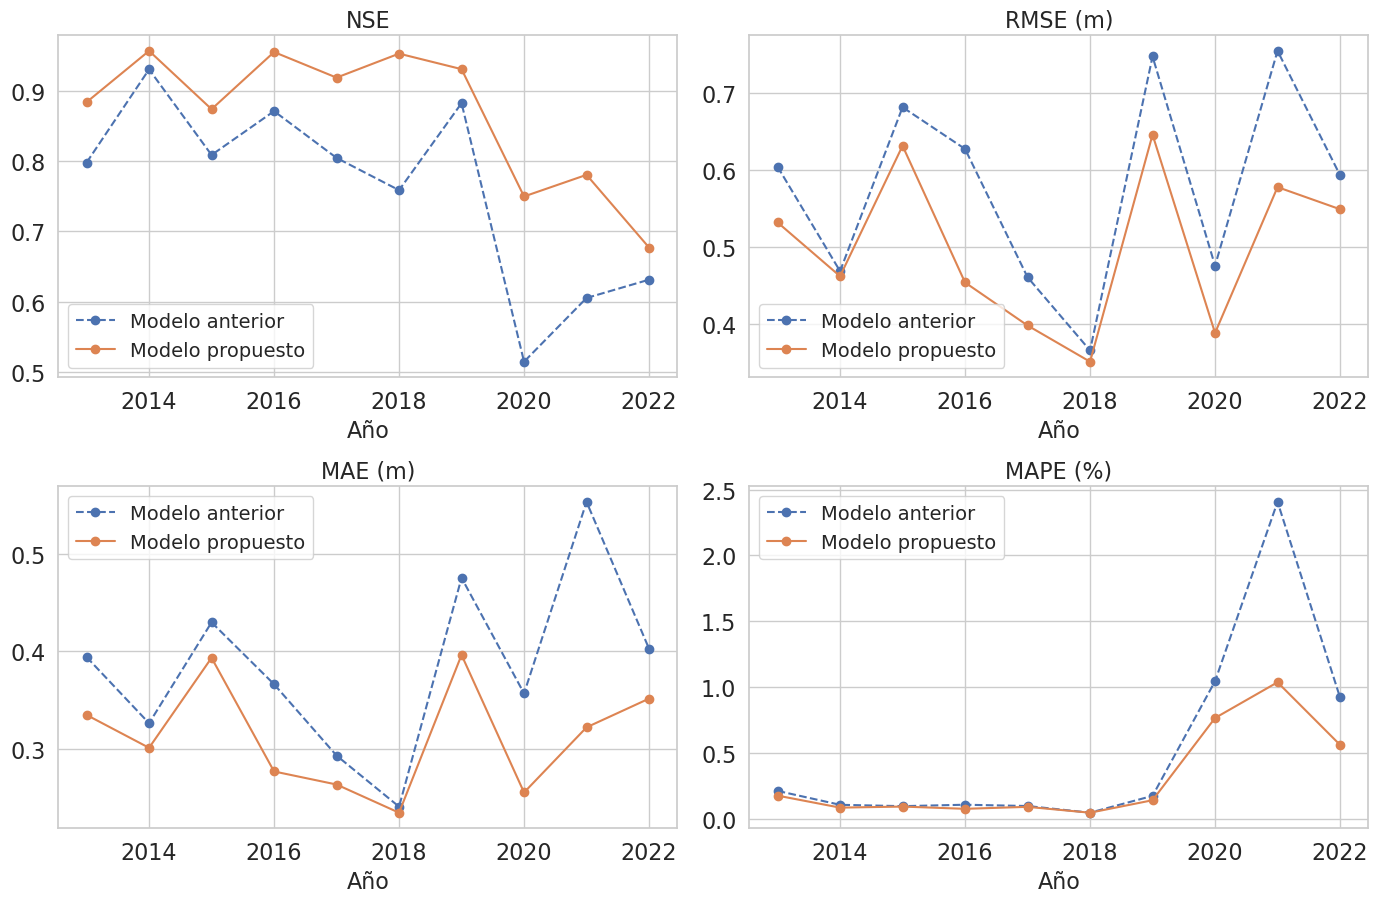
\includegraphics[width=0.95\textwidth]{Figuras/FIGURA_ERRORES_ANUALES.png}
\caption{Evolución anual de las métricas de error para el horizonte de 28 días: comparación entre modelo base y modelo propuesto.}
\label{fig:errores_anuales}
\end{figure}

En términos generales, el modelo propuesto supera de forma consistente al modelo base en casi todos los años y métricas. Esto es particularmente evidente en los valores de NSE, donde se mantiene por encima de 0.9 en la mayoría de los años, mientras que el modelo base exhibe caídas más pronunciadas, especialmente en 2020. Este comportamiento es especialmente relevante, ya que 2020 y 2021 corresponden a uno de los tramos más desafiantes del registro hidrológico reciente, marcado por una bajante histórica del río Paraguay. A pesar de estas condiciones anómalas, el modelo propuesto mantiene un rendimiento superior en todas las métricas, lo que valida su aplicabilidad incluso en escenarios extremos.

Las métricas de error absoluto —RMSE y MAE— también muestran una reducción sistemática en el modelo propuesto, con menor dispersión interanual. La diferencia es más marcada en 2018 y 2021, años en los que el modelo base presenta picos de error más altos, mientras que el modelo mejorado mantiene un nivel de precisión más estable.

En cuanto al MAPE, se observa una mejora drástica en los años más difíciles (2020 y 2021), donde el modelo base supera el 2.0\% mientras que el modelo propuesto se mantiene por debajo del 1.2\%. Esto sugiere que la arquitectura final logra mantener la precisión relativa incluso en periodos caracterizados por sequías prolongadas y niveles históricamente bajos del río.

Este análisis confirma que las mejoras introducidas no solo reducen el error promedio, sino que también aportan estabilidad a lo largo del tiempo, haciéndolo más confiable para aplicaciones operativas continuas.


\subsection{Análisis por Día Predicho (H28)}
\label{ssec:errores_por_dia}

La Figura~\ref{fig:errores_por_dia} muestra la evolución del error promedio según el día predicho dentro del horizonte de 28 días, comparando el modelo anterior y el modelo propuesto. Se presentan las cuatro métricas principales: NSE, RMSE, MAE y MAPE.

\begin{figure}[H]
\centering
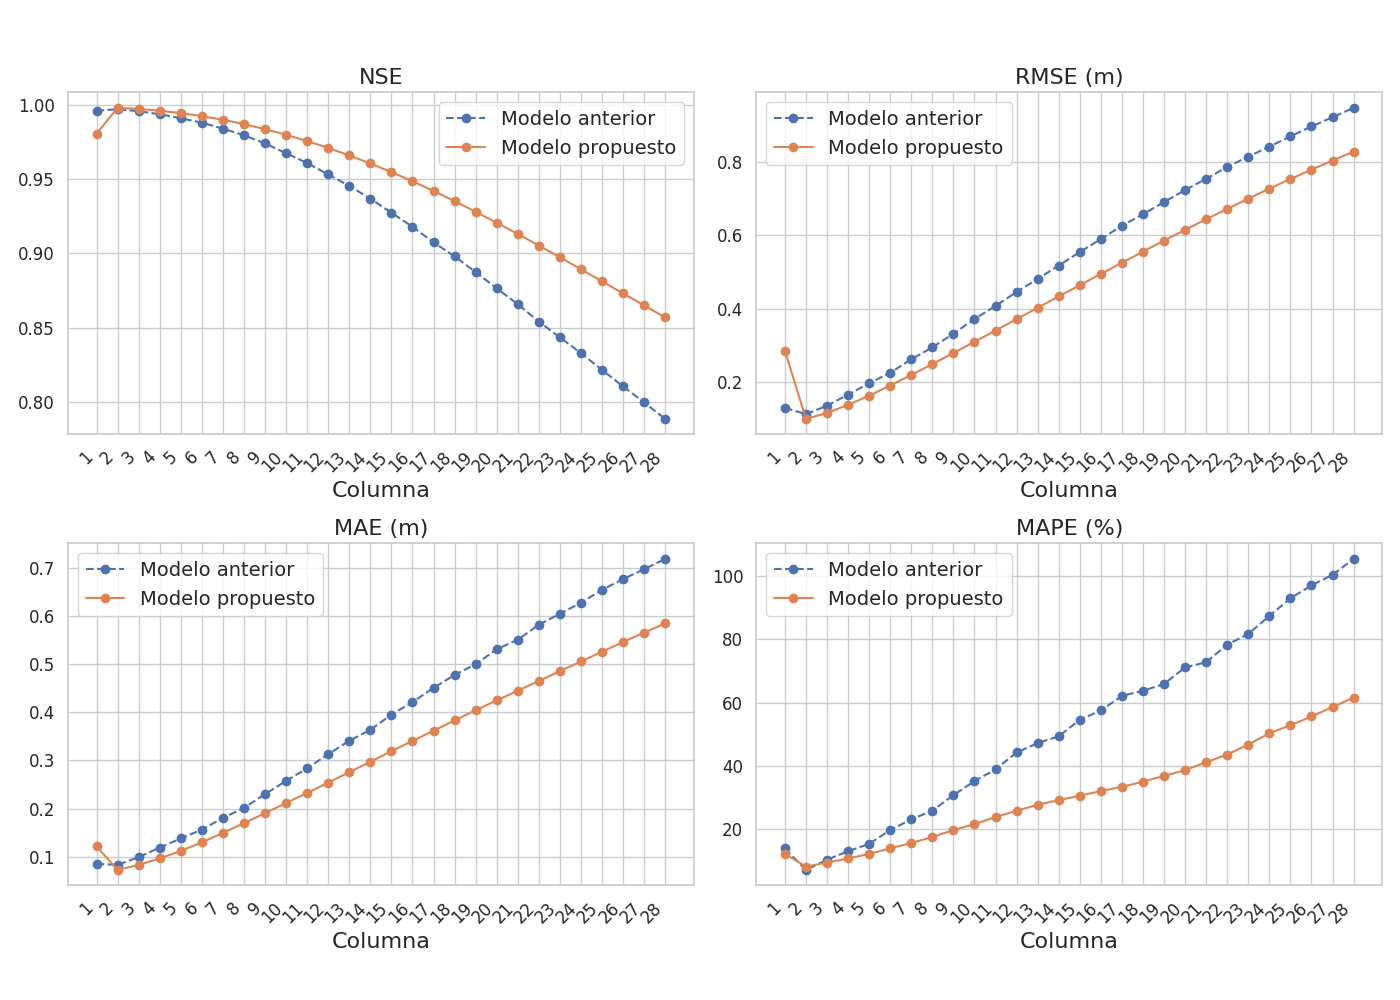
\includegraphics[width=0.95\textwidth]{Figuras/FIGURA_ERRORES_POR_DIA.png}
\caption{Error promedio por día predicho dentro del horizonte de 28 días: comparación entre modelo base y modelo propuesto.}
\label{fig:errores_por_dia}
\end{figure}

Como es habitual en modelos de predicción multi-step, el desempeño disminuye progresivamente a medida que aumenta el día dentro del horizonte. Sin embargo, se destaca que el modelo propuesto logra mantener una pendiente de degradación más suave en todas las métricas evaluadas.

El NSE del modelo propuesto permanece por encima de 0.9 hasta el día 20, mientras que el modelo base cae por debajo de ese umbral a partir del día 13. En cuanto a RMSE y MAE, se observa un crecimiento más contenido en el modelo propuesto, con diferencias acumuladas superiores a 0.15m hacia el final del horizonte. Esta diferencia es crítica, especialmente para decisiones operativas con planificación extendida.

El MAPE también evidencia una mejora sustancial: mientras que el modelo base supera el 100\% de error porcentual en el día 28, el modelo propuesto se mantiene alrededor del 60\%. Esta diferencia refleja una mayor capacidad para anticipar no solo la tendencia, sino también la magnitud del nivel del río a largo plazo.

Este análisis confirma que el modelo propuesto no solo mejora en promedio, sino que también degrada su rendimiento de forma más controlada en predicciones más lejanas, lo cual es un aspecto clave para aplicaciones reales de pronóstico.

\subsection{Comparación estadística de predicciones}
\label{ssec:prueba_dm}

Complementando la comparación visual y las métricas agregadas por horizonte, se aplicó la prueba estadística de Diebold-Mariano (DM)~\cite{diebold1995comparing} para contrastar formalmente la calidad de las predicciones entre el modelo base y el modelo propuesto, en horizontes que van desde 1 hasta 28 días. Esta prueba permite evaluar si las diferencias en los errores de predicción entre ambos modelos son estadísticamente significativas.

Los resultados obtenidos muestran que, salvo en el primer horizonte (día 1), donde el estadístico DM fue de 0.347 con un p-valor de 0.7285 (sin evidencia significativa), el modelo propuesto supera de manera consistente y significativa al modelo base en todos los horizontes subsiguientes. A modo de ejemplo, el estadístico DM alcanza valores de -11.53 en el horizonte 2, -12.36 en el horizonte 12 y -14.71 en el horizonte 28, todos con p-valores menores a 0.0001.

Estos resultados respaldan la superioridad del modelo mejorado conforme aumenta el horizonte de predicción, y validan estadísticamente las observaciones realizadas en la Figura~\ref{fig:errores_por_dia}.


\subsection{Análisis Temporal Detallado}
\label{ssec:zoom_temporal}

La Figura~\ref{fig:zoom_predicciones} muestra un análisis centrado en el periodo comprendido entre enero de 2020 y octubre de 2022, uno de los más críticos dentro del conjunto de prueba. Este tramo se caracteriza por una prolongada bajante del río Paraguay, considerada una de las más severas en más de un siglo. De hecho, en septiembre de 2021, se registró el nivel más bajo del río en Asunción en 117 años, con una profundidad inferior a la mínima operativa para navegación en múltiples tramos \cite{apnews2021,datamar2022}.

\begin{figure}[H]
\centering
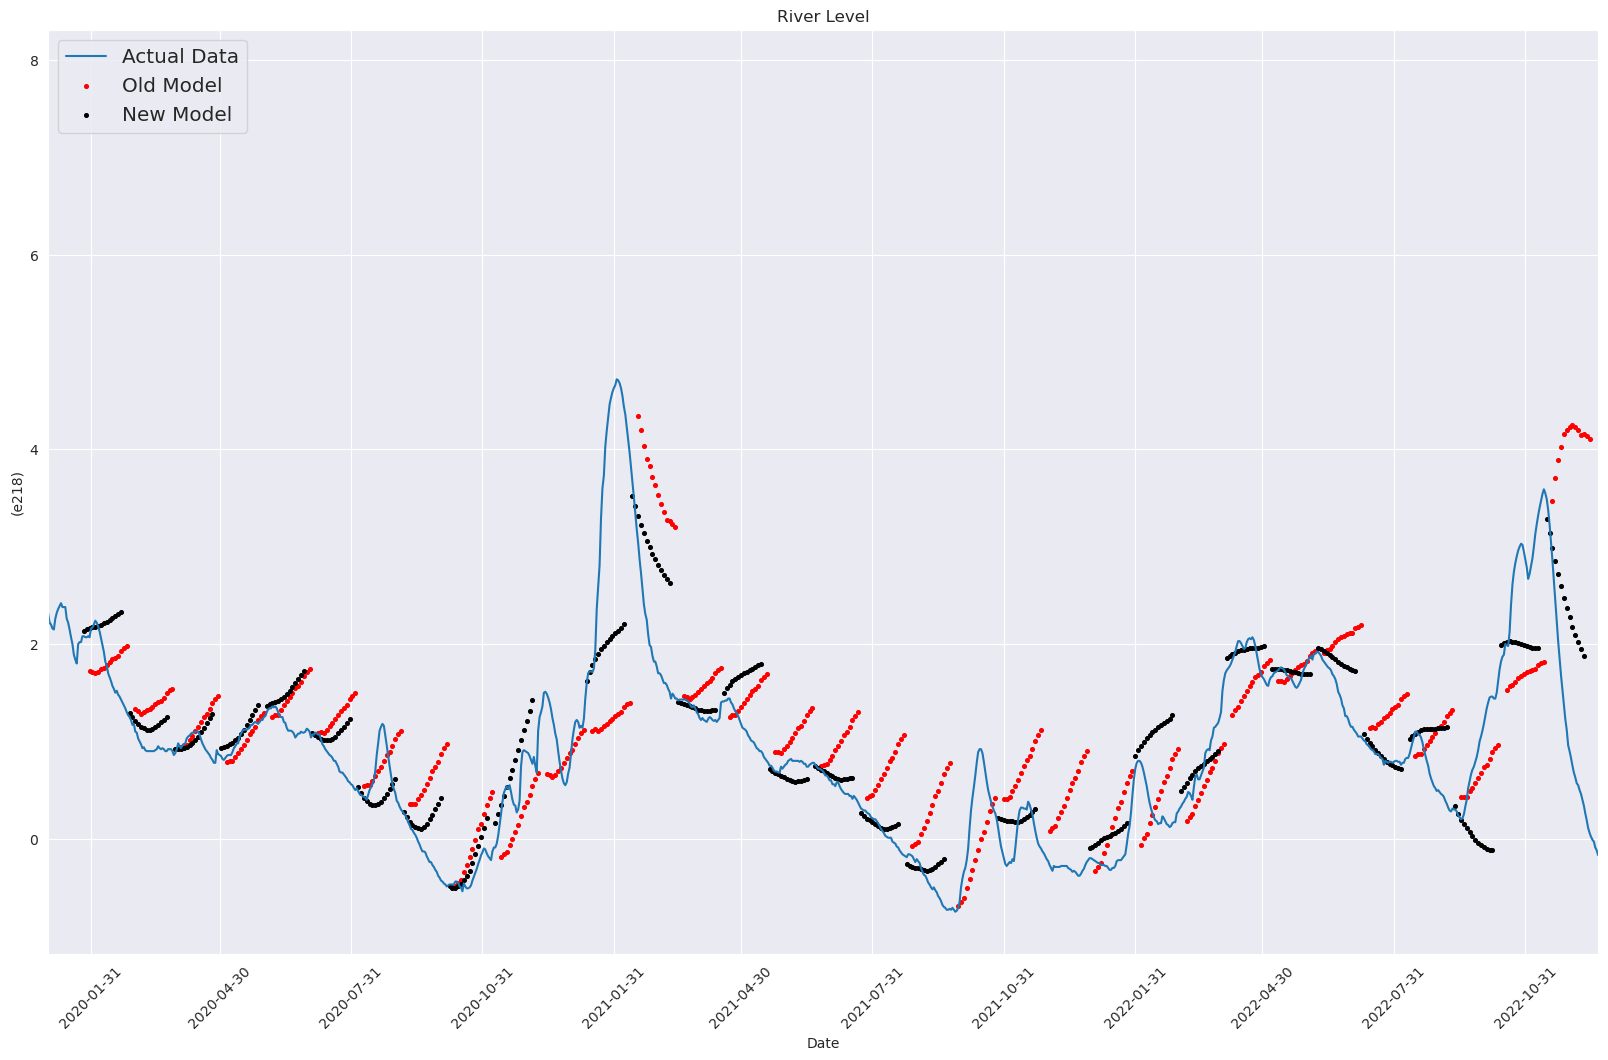
\includegraphics[width=0.95\textwidth]{Figuras/FIGURA_ZOOM_PREDICCIONES.png}
\caption{Zoom sobre el periodo 2020–2022: comparación detallada entre el modelo base (rojo) y el modelo propuesto (negro) frente a la serie real (línea azul).}
\label{fig:zoom_predicciones}
\end{figure}

Este evento hidrológico extremo fue ocasionado por una combinación de factores regionales y climáticos, entre ellos la persistencia del fenómeno La Niña, que redujo las precipitaciones en gran parte de la cuenca del Plata durante tres años consecutivos \cite{datamar2022}. A esto se sumaron impactos indirectos como incendios forestales en zonas ribereñas —incluyendo el Pantanal y el delta del Paraná— y restricciones severas en la navegación fluvial, con efectos económicos y logísticos a nivel nacional \cite{wikiIncendios2020,cih2023}.

Desde el punto de vista de modelado, este periodo representa un desafío significativo para cualquier sistema de predicción. Las condiciones observadas estuvieron marcadas por niveles persistentemente bajos, variabilidad abrupta y eventos puntuales de recuperación o crecida que no siguen patrones estacionales típicos. Esto hace que los modelos entrenados con datos históricos puedan tener dificultades para generalizar correctamente, sobre todo si no se actualizan o enriquecen con variables relevantes.

La visualización muestra que el modelo propuesto (puntos negros) logró adaptarse mejor a estas condiciones adversas. En momentos críticos como el ascenso de principios de 2021, el modelo propuesto fue capaz de anticipar correctamente tanto el inicio como la magnitud del pico, mientras que el modelo base (puntos rojos) presentó una subestimación significativa y mayor dispersión. Del mismo modo, hacia mediados y finales de 2022, cuando se observan oscilaciones más pronunciadas del nivel, el modelo propuesto ofrece predicciones más ajustadas y estables.

Este comportamiento está en línea con las métricas globales presentadas previamente: el modelo propuesto no solo mejora en términos absolutos y relativos (reducción de MAE, MAPE y RMSE), sino que también logra mantener su rendimiento en años con condiciones extraordinarias, como 2020 y 2021. Esto se refleja en la evolución interanual de errores (Figura~\ref{fig:errores_anuales}), donde el modelo base pierde estabilidad de forma notoria, mientras que el modelo propuesto conserva una tendencia mucho más consistente.

En resumen, este análisis puntual permite validar empíricamente la robustez del modelo propuesto, confirmando que las mejoras introducidas —como el reentrenamiento periódico, la incorporación de covariables hidrometeorológicas y la optimización de hiperparámetros— no solo aportan beneficios en condiciones regulares, sino también en contextos operacionales críticos. Esta capacidad de adaptación resulta clave para aplicaciones reales de monitoreo y planificación hídrica, donde los eventos extremos no solo son frecuentes, sino crecientemente relevantes frente al cambio climático.

\subsection{Bandas de Incertidumbre en la Predicción}
\label{ssec:bandas_incertidumbre}

La Figura~\ref{fig:bandas_incertidumbre} muestra las predicciones diarias del modelo final en comparación con los valores observados del nivel del río, junto con bandas de incertidumbre del 95\,\% calculadas mediante la técnica de MC Dropout. Esta estrategia permite estimar la variabilidad inherente a las predicciones del modelo, al realizar múltiples inferencias con diferentes máscaras de dropout activadas durante la etapa de inferencia.

\begin{figure}[H]
\centering

\includegraphics[width=0.95\textwidth]{Figuras/nivel_rio_pred_vs_real_conf95.png}
\caption{Comparación entre las predicciones diarias del modelo propuesto y los valores observados del nivel del río, con bandas de incertidumbre del 95\,\% calculadas mediante MC Dropout (2013–2022).}
\label{fig:bandas_incertidumbre}
\end{figure}

El gráfico permite observar que las bandas de incertidumbre se adaptan dinámicamente a la variabilidad hidrológica: se amplían en periodos más inestables o de transiciones abruptas, y se estrechan en fases de comportamiento más predecible. Este tipo de representación aporta un valor agregado al proceso de toma de decisiones, ya que permite interpretar no solo la predicción puntual, sino también el grado de confianza asociado a cada estimación.

En contextos operativos, esta información puede ser utilizada para definir umbrales de alerta, establecer márgenes de seguridad o identificar ventanas temporales donde la confiabilidad del modelo es menor. Así, el uso de bandas de incertidumbre complementa las métricas tradicionales y fortalece la aplicabilidad del sistema de pronóstico propuesto.